% !TeX root = ../pythonTutorial.tex
\chapter{Steuerung}

Gesteuert wird die gesamte Anwendung mit den Controllern der HTC Vive Pro. Au�erdem wird durch Sensoren im VR-Labor erm�glicht, sich innerhalb des Raumes von drei auf vier Metern (bis zu zehn auf zehn Meter m�glich) frei im Raum zu bewegen. Verwendet man die wireless Variante, erm�glicht dies ein sehr freies und angenehmes Erlebnis. Da man in der virtuellen Realit�t schnell den �berblick verlieren kann, wie weit die jeweiligen W�nde des Raumes noch in Wirklichkeit entfernt sind, wird ein Gitter in der Anwendung angezeigt, wenn man sich dieser zu sehr n�hert. 

Da einer der R�ume f�r die potenzielle Nutzung der maximal m�glichen Raumgr��e entworfen wurde, ist eine Teleport-M�glichkeit unerl�sslich. Diese ist jedoch auch im Flur n�tig und in den anderen R�umen m�glich. Durch Dr�cken des Touchpads des Controllers erscheint ein Marker, den man auf die am Boden befindliche Stelle platzieren muss, an die teleportiert werden soll. Durch Loslassen wird man zur gew�nschten Stelle gebracht.
Die einzige andere Taste, die zur Bedienung verwendet wird, ist der Hairtrigger. Mit diesem lassen sich Gegenst�nde durch Ber�hrung und gleichzeitiges gedr�ckt Haltens des Triggers hochheben. Ein Teleport mit einem aufgehobenen Gegenstand im selben Controller ist nicht m�glich, dazu sind beide Controller notwendig. Mit einem muss man den Gegenstand mit dem Hairtrigger aufnehmen und halten, mit dem anderen wird �ber das Touchpad teleportiert.

\begin{figure}
	\centering
	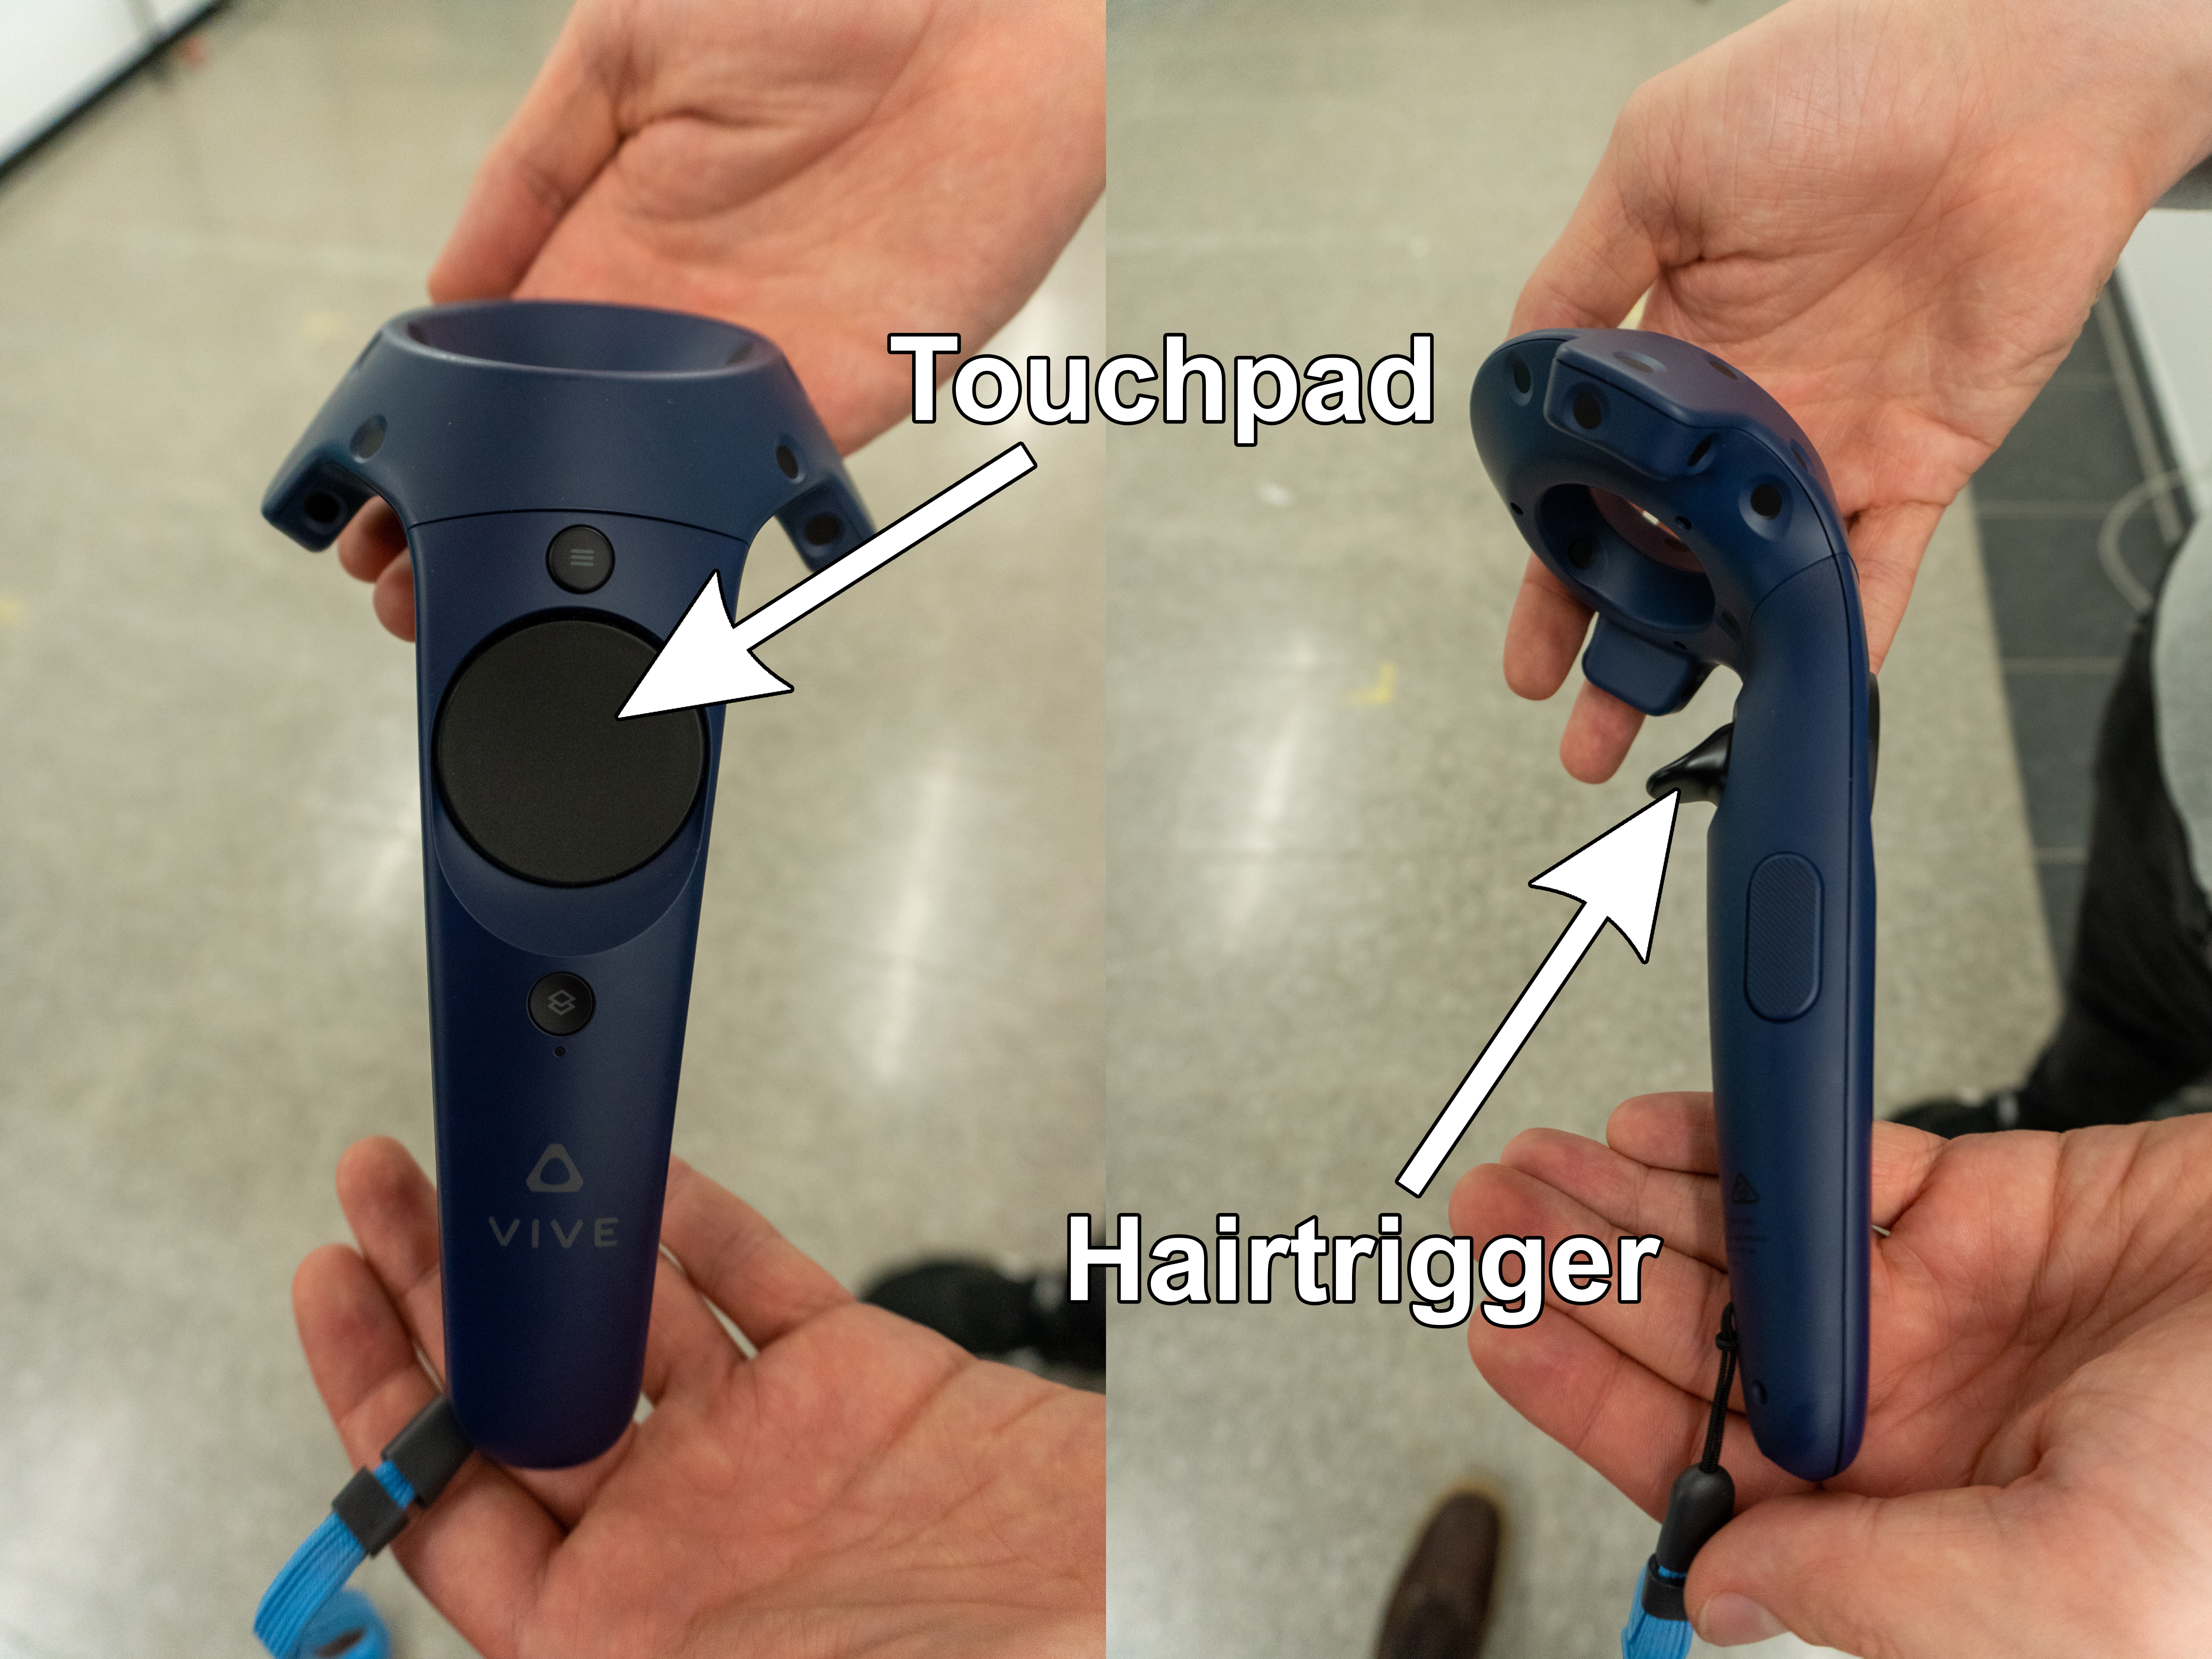
\includegraphics[width=1\textwidth]{images/steuerung/trigger.jpg}
	\caption{Beispiel Controller beschriftet}
	\label{img:controller}
\end{figure}